\appendixsection{Нахождение TKlog в \(\pi\)}

Предположение насчет общей структуры TKlog появилось благодаря наблюдениям за TU-разложением Бирюкова и др.

На Рисунке \ref{fig:figC01} показано TU-разложение $\pi$ и описанные ниже обозначения. Для каждого входа $c$ из $\nu_{1}$, то есть для всех $c \in \mathbb{F}_{2}^{4}$, можно определить два множества $A_{c}$ и $B_{c}$ как
$$
\begin{aligned}
& A_{c}=\left\{\alpha^{-1}(x, x \odot \mathcal{I}(c)), \forall x \in \mathbb{F}_{2}^{4}\right\}, \\
& B_{c}=\left\{\omega\left(\nu_{1}(c), y\right), \forall y \in \mathbb{F}_{2}^{4}\right\} .
\end{aligned}
$$
Множества $A_{c}$ являются векторными пространствами, а множества $B_{c}$ - аддитивные смежные классы векторного пространства $\left\{\omega(0, y), \forall y \in \mathbb{F}_{2}^{4}\right\}$.

\begin{figure}
        \centering
        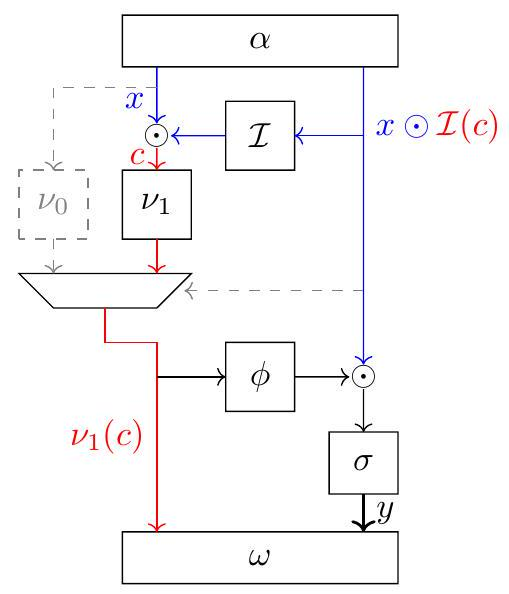
\includegraphics[scale=0.5]{contents/pics/C_pi.jpg}
        \caption{Распространение определенных векторных пространств через \(\pi\)}
        \label{fig:figC01}
\end{figure}

Как видно на Рисунке \ref{fig:figC01}, если применить $\pi$ ко всем элементам $A_{c}$, то получится 16 элементов, из которых 15 принадлежат $B_{c}$. Кроме того, как из Уравнения \ref{eq:01} следует, что $\left\{\alpha^{-1}(x, 0), \forall x \in \mathbb{F}_{2}^{4}\right\}=\left\{\omega(0, x), \forall x \in \mathbb{F}_{2}^{4}\right\}$. Тогда получается, что
$$
B_{c}=\omega\left(\nu_{1}(c), 0\right) \oplus A_{0}
$$
и что $A_{c}$ каким-то образом связано с $A_{0}$ при помощи умножения в конечном поле. Также можно заметить, что эти множества имеют особую связь с матричным умножением, которое используется в Стрибоге. Пусть L - двоичная матрица $64 \times 64$, используемая в Стрибоге, и пусть $[a, 0, \ldots, 0] \times \mathrm{L}=\left[a_{0}^{\prime}, \ldots, a_{7}^{\prime}\right]$. Если $a$ принимает все значения из $A_{c}$ для некоторого $c \in \mathbb{F}_{2}^{4}$, то $a_{i}^{\prime}$ принимает все значения из $A_{c_{i}}$ для некоторого $c_{i}$. Это свойство выполняется независимо от положения $a$ в изначальном векторе. Поскольку из работы Казимрова и Казимровой \cite{KK13} изместно, что L как-то связана с MDS-матрицей с коэффициентами из $\mathrm{GF}\left(2^{8}\right)$, было получено, что множества $A_{c}$ должны иметь определенную связь с этим полем.

Эти наблюдения в сочетании с тем фактом, что $\pi$ каким-то образом связано с логарифмом \cite{PU16}, позволяют сделать предположение, что векторные пространства $A_{c}$ и аффинные пространства $B_{c}$ на самом деле являются соответственно мультипликативными и аддитивными смежными классами единственного векторного пространства размерности 4, которое было быстро определено как подполе.

Эта догадка позволяет написать первое очень грубое разложение $\pi$, которое в дальнейшем итеративно улучшалось путем переписывания его слагаемых все более простыми способами. Конечным результатом этого долгого и утомительного процесса стало разложение $\pi$ в виде TKlog, которое затем было обобщено.